\documentclass[article,a4paper]{IEEEtran}
\usepackage{lipsum}
\usepackage[backend=biber]{biblatex}
\usepackage{graphicx}

\addbibresource{refs.bib}
\title{Data formats, databases and clocks in sync, important for IoT}
\author{
\IEEEauthorblockN{Anton Odén}\\
\IEEEauthorblockA{Dept. of Maths and Computer Science\\Karlstad University\\
651 88 KARLSTAD, Sweden}\\
anton.oden@outlook.com
}

\begin{document}

\maketitle

\begin{abstract}
        dawdadwaw
\end{abstract}

\section{Introduction}
The goal of IoT is to give us data to be able to make informed decisions and let us make decisions that would otherwise never been made but because of IoT is being made and those decisions are contributing to the greater good. In a democratic socitity in a reccurent event every citizen with the right to vote is asked to cast a vote on who should make decisions for the next period. The votes are cast in a ballot box and the votes are counted. All the apparatus around the vote and counting it is a costly operation and in Sweden the authorities of election estimated an reelection to cost 200 million swedish crowns \cite{costElection}. We do it nevertheless because we believe it is an important decision to be made. Thought not every opinion of the citizen has been taken into consideration in that single vote that would give the govermental aparatues the informed knowledge to rule. Alot of other opinions from the citizens would also be beneficial to have gotten voted on to make informed decisions that would otherwise never been made, or that are made but made wrong becuase of lack of information/opinion. Our IoT nodes are also citizens. They are supplying data that could and should help in making informed decisions and just as in politics there is decisions to be made in IoT how close to the end nodes the decision making is to be made. Should all data be communicated to the cloud to be processed there or should the data be processed closer to the end nodes? The answer to that question is not easy and there are many factors to take into consideration. One of the factors is the time it takes to communicate the data to the cloud and back. Another is the bandwidth of the communication channel taken up when all things communicate on it. The highways has to be broadened to the able to take the load and there is costs associated with that. This article will...
\section{Data formats}  
The payload needs to be communicated in a data format that both reiciever and transmitter knows how to work with. On gateways and servers that has bigger capabilities with memory and compute a complicated data format is no problem. But on small end devices, especially those that run on battery, the dataformat needs to be lightweight.
\newline\newline      
JavaScript Object Notation (JSON) is THE dataformat of IoT communication. It doesn't have to be JSON but it has become a standard and is used in many applications and originally known in data transmission between server and client for webpages, hence the Javascript part and it's an international industry standard (ECMA-404) \cite{JSONstandard}. JSON is lightweight, easy for humans to read, completely language independent and thereby used in many programming languages for data interchange\cite{JSONintro}. JSON makes use of bracket signs to envelope data in objects and can nest data in hierarchies this way. Label and data is separated by a colon and both parts are enveloped by quotation signs. The labeling text could be made as short as one sign and a separate JSON Schema could contain more specified information regarding the data \cite{JSONformat}. The schema is shared between transmitter and reiciever and is used for validation of the data in parsing. For minimal bandwidth usage it's a good idea to make labels short and let the commonly known schema act as a translater to make the code more readable.
\begin{figure}
    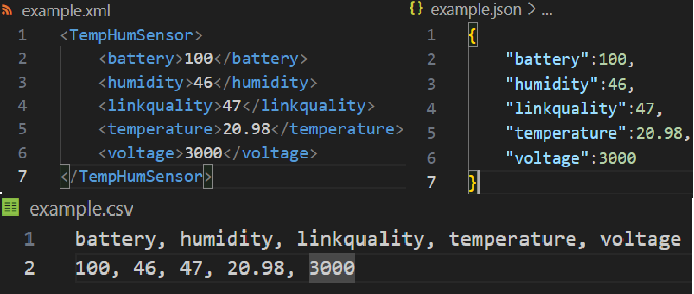
\includegraphics[width=\columnwidth]{JSON-XML-CSV.png} 
    \caption{ Example: XML up-left, JSON up-right, CSV down }
    \label{fig1:XML and JSON example}   
\end{figure}   
\newline\newline
\cite{XMLdocs}Extensible Markup Language (XML) is another common data format for data interchange and is influenced by html in its hierarchical structure where each piece of data (entity) is enclosed within a descriptive tag forming a tree structure that mirrors the relationships between the different entities. As seen in fig1 XML needs opening and closing tags to envelope it's data compared to JSON. It is also dependent on more complex parsing as it allows tags to be given attributes and namespaces to be set to avoid conflicts. This is a problem for IoT devices that needs transmission time to be set to a minimum to not consume battery and it also takes more bandwidth on the network. There are some built in security in XML that does give it some egde in that certain parts of the data could be restricted by further encryption being benificial in a world of documents \cite{XMLSecurity}. But in IoT where the chunk of data from sensors and actuators is relativily small an encryption on top of all data is probably enought.    
\newline\newline
\cite{CSVdocs}Comma Separated Value (CSV) is a data format that explain itself in its name, every block of data (value) is divided by a comma, as can be seen in fig1. First line in this format optionaly contain an header for the data and then each line represent a new set of data. It is a standard since 2005 but originates from before personal computers. The data format is excellent for spreedsheets and the overhead is minimal. A problem thought is that other than headerpart that act as labels, CSV files lack the capability for hierarchy, metadata, datatypes and other structures that JSON and XML has. 
\newline\newline
JSON as we already discussed is the most comon used data format in IoT and as could be seen i fig2 the trend overall in all applications is that JSON is taking shares as XML drastically has shrinken in usage since 2004.  
\begin{figure}
    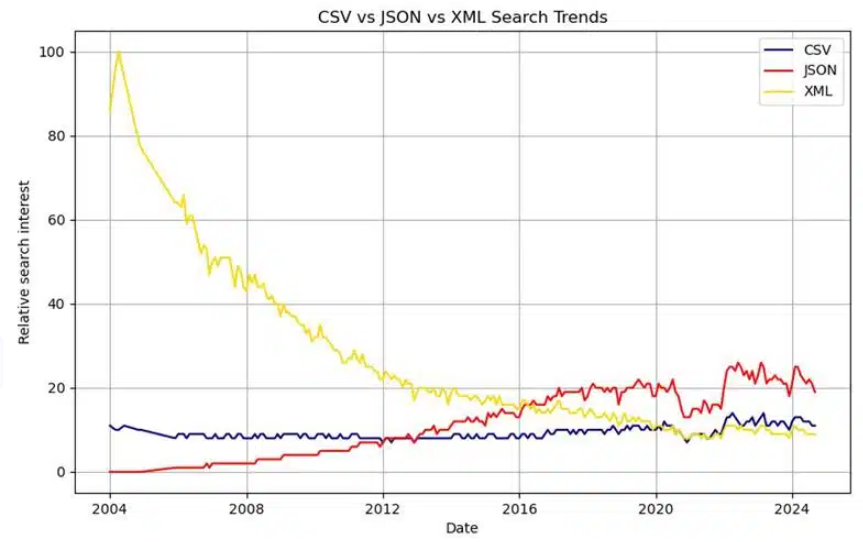
\includegraphics[width=\columnwidth]{DataFormatTrend.png} 
    \caption{ Trend showing rise of JSON compared to XML \cite{CompareJSONXMLCSV} }
    \label{fig2: Trend XML CSV JSON }   
\end{figure}
\section{Clock Syncronization}
A data that is important for most smart decisionmaking, retrospective analysis etc. is time. To have an acccurate knowing of time a certain event occured syncronization of clocks is needed. Every IoT device has its own idea of the current time amd clocks drifts as they are derived from an oscillators frequency. The frequency has manufacturing variability and is influenced by aging, temperature and overdrive so it is difficult for devices to recalculate it's clock by themself. Sensors in IoT in for example the LoRaWAN protocol has the capability to hibernate to conserve battery. To have different knowing of time can do that the server for example thinks a sensor is listening for transmission on a certain time being class Beacon device. Thereby a network clock syncronization protocol is needed for the IoT network (and other networks too). 
\newline\newline 
\cite{NTPv4}Network Time Protocol (NTP) was standardized in 1985 (RFC958) and is now envolved into version 4, published 2010 (RFC5905), being backwards compatible. An NTP network is in hierarchy with the root being stratum 0 that contain a few atomic clocks with superprecise time. A few time servers are allowed to communicate with stratum 0 formning stratum 1 and the stratum number increases depending on how many time server jumps the device is from stratum 1. The server or device being closest to stratum 1 in hierchy and nearest in time from syncronization has the most accurate time. In an IoT network it may be unnessary for all sensors to have an exact knowledge of the time but what's important is that all the devices within the local network being able to communicate are at syncronization with eachother. 
\newline\newline
The Berkeley algorithm \cite{Berkleyalgo} solves this by assigning one node within the network master status. The masternode is responsible to periodically fetch clock time from all nodes within network. The masternode then calculate an average time between all the nodes, updates its own clock then broadcasts the time over the network for all nodes to update their clocks. Berkley algorithm is a good fit to keep IoT devices within a local network in syncronization and then in wider periods the masternode could fetch timeupdates from closest stratum using NTP to keep the local network relativily synced with global world time.  
\newline\newline
Latency within the network has been taken into consideration for the masternode in Berkley algorithm to be able to calculate correct average time. This is done via Cristians algorithm as all devices can't be assumed having the same round trip time (RTT). In fig3 client is masternode and server is the nodes that the masternode periodically fetches clock times from \cite{Christianalgo}. 
\begin{figure}
    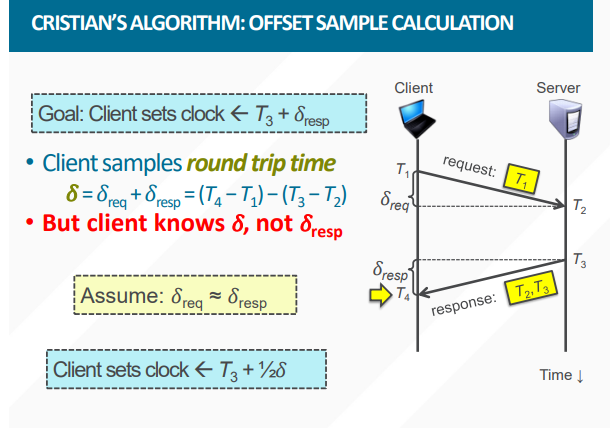
\includegraphics[width=\columnwidth]{Cristianalgo.png} 
    \caption{ Snapshot from slide in \cite{Timesyncslides} }
    \label{fig3: Cristianalgo }   
\end{figure}
\section{Data storage}
All data that is being sent needs a space to be stored. Throught the network it is stored in fast and small memory close to data processing units deciding where the data is to be stored next. Data is packaged, transmitted, depackaged, processed, packaged, transmitted, depackaged, processed etc. At some point the data stored in a bigger storage called database. Databases have historicly been relational databases that are structured where similar to spreedsheets discussed in CSV section. Data is attached to a table that the data has the closest relation to, having other data in the same table also having the closest relation to eachother. 
\newline 
Then relationsships is built up between tables via unique keys that could in themself be formning another relationsshiptable. This kind of structure does the job when data labels doesn't change or new labels of data isn't added to often. It is said that they scale vertically well, meaning alot of data of the same kind. But lack when it comes to scaling horizontally, meaning adding to much columns to the tables is more stressful for containing order in the structure of a relational database. Relational databases is categories as SQL-databases as SQL (Structured Query Language) is deeply attached to relational databases being the most common language used communicating with an relational database. NoSQL databases is united is that they are non-traditional relation databases. Some categories on NoSQL databases are key-value, document, wide-column \cite{Databasesurvey}, graph and time-series databases.      
\newline\newline
Key-value databases is formed as a long list with keys that each on points to a certain value. Just like a memory registry where every adress contain some binary data. In a key-value store the value part is not as in a memory registry restricted to a specific memorysize, in a key-value store the value could be anything. Key-value excel when in comes to looking up specific data fast cause the keys can be in sorted order making binary searching the database possible. 
\newline\newline
Building on top of key-value is another category called document databases that are similar but with availability to search the valuepart. Giving filtering and more complex queries availability to the database. Documents are structured in a XML or JSON manor that makes the transition between storing and transmission of data quick and easy to implement for system development. 
\newline\newline
Wide-column databases  
\printbibliography

\end{document}